
%%\documentclass[preprint,12pt]{elsarticle}

%% Use the option review to obtain double line spacing
\documentclass[preprint,review,12pt]{elsarticle}

%% Use the options 1p,twocolumn; 3p; 3p,twocolumn; 5p; or 5p,twocolumn
%% for a journal layout:
  %% \documentclass[final,1p,times]{elsarticle}
%% \documentclass[final,1p,times,twocolumn]{elsarticle}
%% \documentclass[final,3p,times]{elsarticle}
%% \documentclass[final,3p,times,twocolumn]{elsarticle}
%% \documentclass[final,5p,times]{elsarticle}
%% \documentclass[final,5p,times,twocolumn]{elsarticle}

%% if you use PostScript figures in your article
%% use the graphics package for simple commands
%% \usepackage{graphics}
%% or use the graphicx package for more complicated commands
%% \usepackage{graphicx}
%% or use the epsfig package if you prefer to use the old commands
%% \usepackage{epsfig}

%% The amssymb package provides various useful mathematical symbols
\usepackage{amssymb}
%% The amsthm package provides extended theorem environments
%% \usepackage{amsthm}

%% The lineno packages adds line numbers. Start line numbering with
%% \begin{linenumbers}, end it with \end{linenumbers}. Or switch it on
%% for the whole article with \linenumbers after \end{frontmatter}.
\usepackage{lineno}

%% natbib.sty is loaded by default. However, natbib options can be
%% provided with \biboptions{...} command. Following options are
%% valid:

  %  round  -  round parentheses are used (default)
%  square -  square brackets are used   [option]
%  curly  -  curly braces are used      {option}
%  angle  -  angle brackets are used    <option>
  %  semicolon  -  multiple citations separated by semi-colon
%  colon  - same as semicolon, an earlier confusion
%  comma  -  separated by comma
%  numbers-  selects numerical citations
%  super  -  numerical citations as superscripts
%  sort   -  sorts multiple citations according to order in ref. list
%  sort&compress   -  like sort, but also compresses numerical citations
%  compress - compresses without sorting

\biboptions{comma,square}

% \biboptions{}
\usepackage{textcomp, fixltx2e}
\usepackage{fullpage, lscape}

\journal{Journal of Analytical and Applied Pyrolysis}
\usepackage{Sweave}
\begin{document}

\begin{frontmatter}

%% Title, authors and addresses

%% use the tnoteref command within \title for footnotes;
%% use the tnotetext command for the associated footnote;
%% use the fnref command within \author or \address for footnotes;
%% use the fntext command for the associated footnote;
%% use the corref command within \author for corresponding author footnotes;
%% use the cortext command for the associated footnote;
%% use the ead command for the email address,
%% and the form \ead[url] for the home page:
  %%
%% \title{Title\tnoteref{label1}}
%% \tnotetext[label1]{}
%% \author{Name\corref{cor1}\fnref{label2}}
%% \ead{email address}
%% \ead[url]{home page}
%% \fntext[label2]{}
%% \cortext[cor1]{}
%% \address{Address\fnref{label3}}
%% \fntext[label3]{}

\title{Following beech litter decomposition with analytical pyrolysis: Inter-site variance and decomposition trends}

%% use optional labels to link authors explicitly to addresses:
  %% \author[label1,label2]{<author name>}
%% \address[label1]{<address>}
%% \address[label2]{<address>}

\author{}

\address{}

\begin{abstract}
%% Text of abstract

Litter decomposition studies are key to understanding global carbon fluxes and soil formation. Analytical pyrolysis has the potential to provide insight into carbon transformations during decomposition. Most interestingly, this potential was not exploited yet. 
We report data of beech litter pyrolysis products of litter optained from different sites in Austria and changes in pyrolysis products during litter decomposition

\end{abstract}

\begin{keyword}
%% keywords here, in the form: keyword \sep keyword

%% MSC codes here, in the form: \MSC code \sep code
%% or \MSC[2008] code \sep code (2000 is the default)

\end{keyword}

\end{frontmatter}
%\pagestyle{empty}
\linenumbers

\section{Introduction}

Understanding plant litter decomposition processes is key to understanding the global carbon cycle, nutrient recycling and soil formation\citep{Prescott2010}. However, little is known about changes in the chemistry of high molecular weight substances during decomposition. The insufficient specifity of traditional methods to determine plant fibres\citep{Hatfield2005} led to misinterpretation of decomposition dynamics. Analytical pyrolysis can provide and fast a cheap method to investigate chemical transformations of plant polymers during decomposition. However, while the use of analytical pyrolysis to quantify lignin and cellulose contents becomes more frequent, the full potential of an high definition interpretation of pyrograms is rarely used.

Analytical pyrolysis is frequently applied to characterize natural organic polymers in soil organic matter [and dissolved organic matter?]. Plant derived compounds make up an important part of pyrolysis products found. The relative abundances of such markers were shown to hold key information on past climates and decomposition conditions \cite{Kuder1998, Schellekens2009, Schellekens2011}.

Only a handful of Pyr-GC/MS studies tracing changing pyrolysis markers during litter decomposition were published, none of them includes indepth. The only published work directly studying the decay of plant leaf litter is \cite{Franchini2002}. \cite{Snajdr2010} presents basic thermochemolysis data.  Straw was incubated with n. Several studies monitor the decomposition of woody material with Pyr GC/MS [lit.] or litter/soils mixtures[lit.]. None of the studies mentioned above analysis decomposition trends of individual pyrolysis products.

While assignment to major compounds classes (like ligin or carbohydrate) based on pyrolysis reaction mechnisms is common, little is known on whether the composition of individual pyrolysis products within this groups yields information.

This study compares pyrograms of beech litter from different site after up to 15 month of climate chamber decomposition. Beech litter were reported for exceptionally slow decomposition rates (12\% mass losso in the first year) in nature \citep{Klotzbucher2007} and showed similar decomposition rates our climate chamber experiment. Therefore, we do not focus on the accumulation of recalcitrant compounds, but focus on how individual pyrolysis markers accumulate or deplete relative to their compounds of origin which might provide insight into changes in polymer condensation patterns.

\section{Material and Methods}

Beech litter from 4 different sites in Austria was collected in October 2008, cut to pieces \textless 0.5 cm, homogenized, sterilized and inoculated with a common inoculate for all sites. Litter was incubated in a climate chamber at 15 \textdegree C and was kept at 60 \% moisture \citep{Wanek2010}. Total mass loss after 15 month was between 7 and 12 \%. Accumulated respiration after 6 month accounts for nn.to nn\% of the litter carbon pool, after 15 month between n and n.

Pyrolysis-GC/MS was performed on a Pyroprobe 5250 pyrolysis system (CDS Analytical) coupled to a Thermo Trace gas chromatograph an a DSQ II MS detector (both Thermo Scientific) equipped with a carbowax colomn (Supelcowax 10, Sigma-Aldrich). 2-300 \textmu g dried and finely ball-milled litter were heated to 600\textdegree C for 10 seconds in helium atmosphere. The temperature of the valve oven and the transfer line to the GC injection port were set to 250\textdegree C,a 10x split injection was applied with the injector heated to 240\textdegree C. Carrier gas flow was set to 1ml min$^{-1}$. GC Oven temperature was constant at 50 \textdegree C for 2 minutes, followed by an increase of 7\textdegree C/min to a final temperature of 260 \textdegree C, which was held for 15 minutes. The transfer line was heated to 270 \textdegree C. The MS detector was set for electron ionization at 70 EV, the ion source was heated to 270\textdegree C. Detection was set to cycle between m/z 20 and 300 with a cycle time of 0.3 seconds.


Peaks were assignment was based on NiSt 05 MS library and comparison with reference material measured.  128 peaks were selected for integration due to their hiht abundance or diagnostic value. For each peak between one and four mass fragments selected for high abundance and specificity were integrated (i.e. \cite{Schellekens2009}). Peak areas are stated as \% of the sum of all integrated peaks of a sample. 

Pyrolysis products were assigned to their substances of origin by comparison to reference material, structural similarity and in accordance with literature (\cite{Ralph1991a, Schellekens2009, Chiavari1992}[more lit!]). We confirmed the identity of two products rarely reported for plant material (Phytol and 3-Hydroxypyridine) by the addition of reference material to the sample and comparison to MS libraries. Both substances were bought from Sigma-Aldrich (St. Louis, MO, USA).

%The sum of all peak areas of the pyrolysis products of a class was calculated based on total ion current (TIC) peak areas. TIC peak areas are (1) less specific as areas of specific MS fragments and (2) integration was not possible for all peaks a/o all samples. Therefore a MS response factor Rf was calculated for each detected substance:
  %
%\begin{equation}
%Rf = median (\frac{TIC peak area}{specific MS fragment peak area})
%\end{equation}
%
%Peak areas were multiplied by Rf before addition to calculate percentages of TIC area without loosing the specifity of integrating single m/z traces \citep{Kuder1998}.
%
% However, during interpretation, we found little difference between direct sums of the integrated fragments and sums of corrected areas, indicating little sensitivity for exact
%
%Relative peak areas in both integrations are different from weight\%, but allow tracing of accumulation/depletion of these substance classes during decomposition \citep{Kuder1998}.
%
%Percent of the initial content lost during decomposition were calculated according to

\begin{equation}
\% lost = \frac {mean()actual \%)} {1-\frac{carbon respired}{initial carbon content}} - \% mean initial content
\end{equation}

\subsection{Litter mass loss and respiration}

\subsection{Statistical analysis}
All statistical analyses were performed with the software and statistical computing environment R using the R package ``vegan'' \citep{Oksanen2011}. If not mentioned otherwise, results were considered significant, when p\textless 0.05. All correlations refer to Pearson correlations.
All data presented was tested for significant differences between harvests and litter types. Normal distribution assumed but could not be tested due to the small number of cases per treatment (n=4-5). A substantial part of variables had heterogeneous variances when tested ẃith Levene's test. Therefore, (one-way) Welch anova was used to calculate significant differences between harvests within each litter type and litter types within each harvest (alpha=0.05). For post-hoc group assignment, paired Welch's t-tests with Bonferroni corrected p limits were used. Principal component analysis was performed using vegan function ``rda'' scaling variables.

\section{Results}

\subsection{Mass loss and respiration}

Accumulated mass loss during the first 181 days ranged between

\subsection{Pyrolysis products}


A total of 128 peaks quantified including 28 phenolic, 11 nitrogen containing compounds and 42 carbohydrate derived compounds. Inter-site differences dominate both initial and incubated litter: In 127  peaks significant differences between litter from different sites was found during one time point, in 95 differences were significant in all 4 harvests. In 113 peaks significant differences between time points were found, but only 49 peaks had significant changes during incubation in more than two litter types.
%Our chromatography system using a carbowax column allows to measure some more hydrophilic compounds (i.e. Pyridol), on the other hand we miss several




\subsection{Lignin and other phenolic compounds}
Of 38 phenolic pyrolysis products were identified, 15 of which had guaiacol-, 13 syringol-, and 10 non-methoxylated ring systems.

Guaiacol/Syringol (G/S) ratios were tightly (all R=0.68-0.94, p<0.001) correlated between the more abundant side chains (-H, -CH$_3$, -CH$_2$CH$_3$, -CH=CH$_2$, -CH$_3$CH=CH$_2$). This correlation is weaker or non-significant for less abundant side chains (-CHO, -CH$_2$CH$_2$CHO) due to higher variances in their detection.

Part of non-methoxylated phenols pyrolysis products (side chains -CH$_2$CH$_3$, -CH$_2$CH$_2$CH$_3$ -CH$_3$CH=CH$_2$)show clear structural similarity to pyrolysis products of lignin, suggesting that they are pyrolysis products of p-hydroxypropanylphenol based lignin. Other side chains (-H, -CH$_3$, -CHO) are less specific and are reported for other sources, although in small amounts. Furthermore, some of the phenolic compounds (i.e. hydroxyquinone) are not lignin derived.

In both syringol and gaiacol the ratio between the abundances of pyrolysis products is the same.

Guaiacol to Syringol ratios were constant over decomposition time. The ratios are are different for G/S compounds with different side chains, propably due to changing MS resposes of the compounds

Most important difference between sites were observed in the ratio between Guaiacol

The pattern of abundances of different side chains was the same for guaiacol and syringol derived compounds. Fig \ref{fig:sidechainratios} shows that pairwise ratios between 5 different lignin side chains are highly significant in guaiacol and syringol lignin based pyrolysis products. However, there are some site-specific differences in these patterns: the abundance of -H and -CH$_3$ side chains relative to other side chains is different between the litter types, but consistent between guaiacol and syringol derivatives.
de chains with oxygen based functional groups were present, but in abundances much lower than the before mentioned.


\cite{Kuder1998, Schellekens2009} use the Guaiacol+Syringol to C$_3$-Gaiacol+Syringol ratio as an indicator for ?aerobic/anaerobic degradation. 

\subsection{N compounds}


In total, 11 nitrogen containing compounds were identified, including two indole three pyridine and 5 pyrrol derrivatives. 8 of them were stricly correlated to litter N content (all R\textgreater 0.8, p\textless 0.001).Two groups could be identified amoung them: indol and methylindole were highly correlated to each other (R=0.98, p\textless 0.05?0.001?), as were 6 pyridin and pyrrol derivatives (all R \textgreater 0.9, p\textless 0.05?0.001?). Correlations between peaks of two groups were still high, but lower than within the groups (R = 0.77-0.87, p\textless 0.05?0.001?). Both groups show a continuous increase during litter decomposition: after 15 month pyridine and pyrrol derrivatives increase by 8-20\% of their initial content, indol and methylindol by 20-30\% (fig. \ref{fig:npeaks}).

Two pyrolysis products show different trends:  The abundance of 3-Hydroxypyrrol strongly (30-50\%) decreases during first six month, then follows general N trend. N-methyl-pyrrol shows an increase between 5 and 35\% (\%TIC) during the first 6 month and remains stable thereafter (fig. \ref{fig:npeaks}).

\subsection{Carbohydrates}
In total, 42 carbohydrate derived pyrolysis products were identified either by their structure or by comparison to reference material %(cellulose, xylan, glucose, ...).
Unlike lignin or N compounds, carbohydrate pyrolysis products do not follow a common trend, but - reflecting the differences within this group. About a third of the peaks could not be identified but were assigned to carbohydrates because they are present reference pyrograms of cabrohydrates, but not in other compounds.

Methylated cyclopentenone derivatives show an increase over decomposition, while derivative with keto- or hydroxy- side chains show decreases over decomposition.

Furanmethanol shows an especially high degradation rate, loosing 15 to 30 \% of it's initial contribution to the total peak area over 15 month.


\subsection{Other compounds}
\subsubsection{Phytol}
 
We found two compounds with terpenoid structure: Phytol is a chlorphyll derived C$_{20}$ alcohol  mentioned as a pyrolysis product only by \cite{Schwarzinger??}. We confirmed the compounds identity by comparison with comercially available material. Phytol is strongly depleted during decomposition in low-N sites (up to 50\% of its relative peak area in OS and AK), but not in high-N sites (SW). (fig \ref{fig:notlignin})



%and a second one identified as Limonene by the NiSt data base. 

\subsubsection{Fatty acids}
Three saturated fatty acids were found in litter pyrograms (14:0, 16:0, 18:0). The three fatty acids were also most abundant in THM analysis of this litter material (data not shown).

%For fatty acid analysis 2 samples were excluded as contaminations were encountered.

Initial content of fatty acids showed differences of up to 30 \% between sites.
Fot the three fatty acids found, between 15 and 50 \% were degraded over 15 month, indication that both accumulation and depletion occurs in certain sites.

\subsubsection{Long chained alkanes and alkenes}

We found C25-C29 alkanes and alkenes in our pyrograms. The two had different decomposition trends: While

\section{Discussion}

\subsection{Inter-site variance during litter decomposition}
We found that differences in litter pyrolysis products persist at least during early litter decomposition. Differences in Lignin side chains indicate different polymerization patterns in different sites. 

\subsection{Lignin side chains}
Until now, studies following lignin degradation with Pyr-GC/MS were focusing on changes between the frequency of lignin pyrolysis products, only the ratio between guaiacol/syringol/phenol based ring system was investigated. We found substantial differences in the frequency of different lignin side chains between litter collected at different sites. We found that these differences remained nearly constant during during 15 month of litter decomposition.

\subsection{Pyridine/Pyrrol to Indole ratio}

The ration between indene and pyridine/pyrrol ring pyroylsis products drops during decomposition by about 20\%. Initial differences between sites (OS is higher than the rest) remain.
Increase in tryptophan content among amino acids in bacterial protein?

\subsection{Lipophilic compounds}

From our dataset, we see that (1) alcenes are accumulated

\section{Conclusions}


\section{Acknowledgements}

%% The Appendices part is started with the command \appendix;
%% appendix sections are then done as normal sections
%% \appendix

%% \section{}
%% \label{}

%% References
%%
%% Following citation commands can be used in the body text:
%% Usage of \cite is as follows:
%%   \cite{key}          ==>>  [#]
%%   \cite[chap. 2]{key} ==>>  [#, chap. 2]
%%   \citet{key}         ==>>  Author [#]

%% References with bibTeX database:

\bibliographystyle{elsarticle-num}
\bibliography{library}



\newpage
\begin{figure*}[h!]
\begin{center}
\setkeys{Gin}{width=0.5\textwidth}
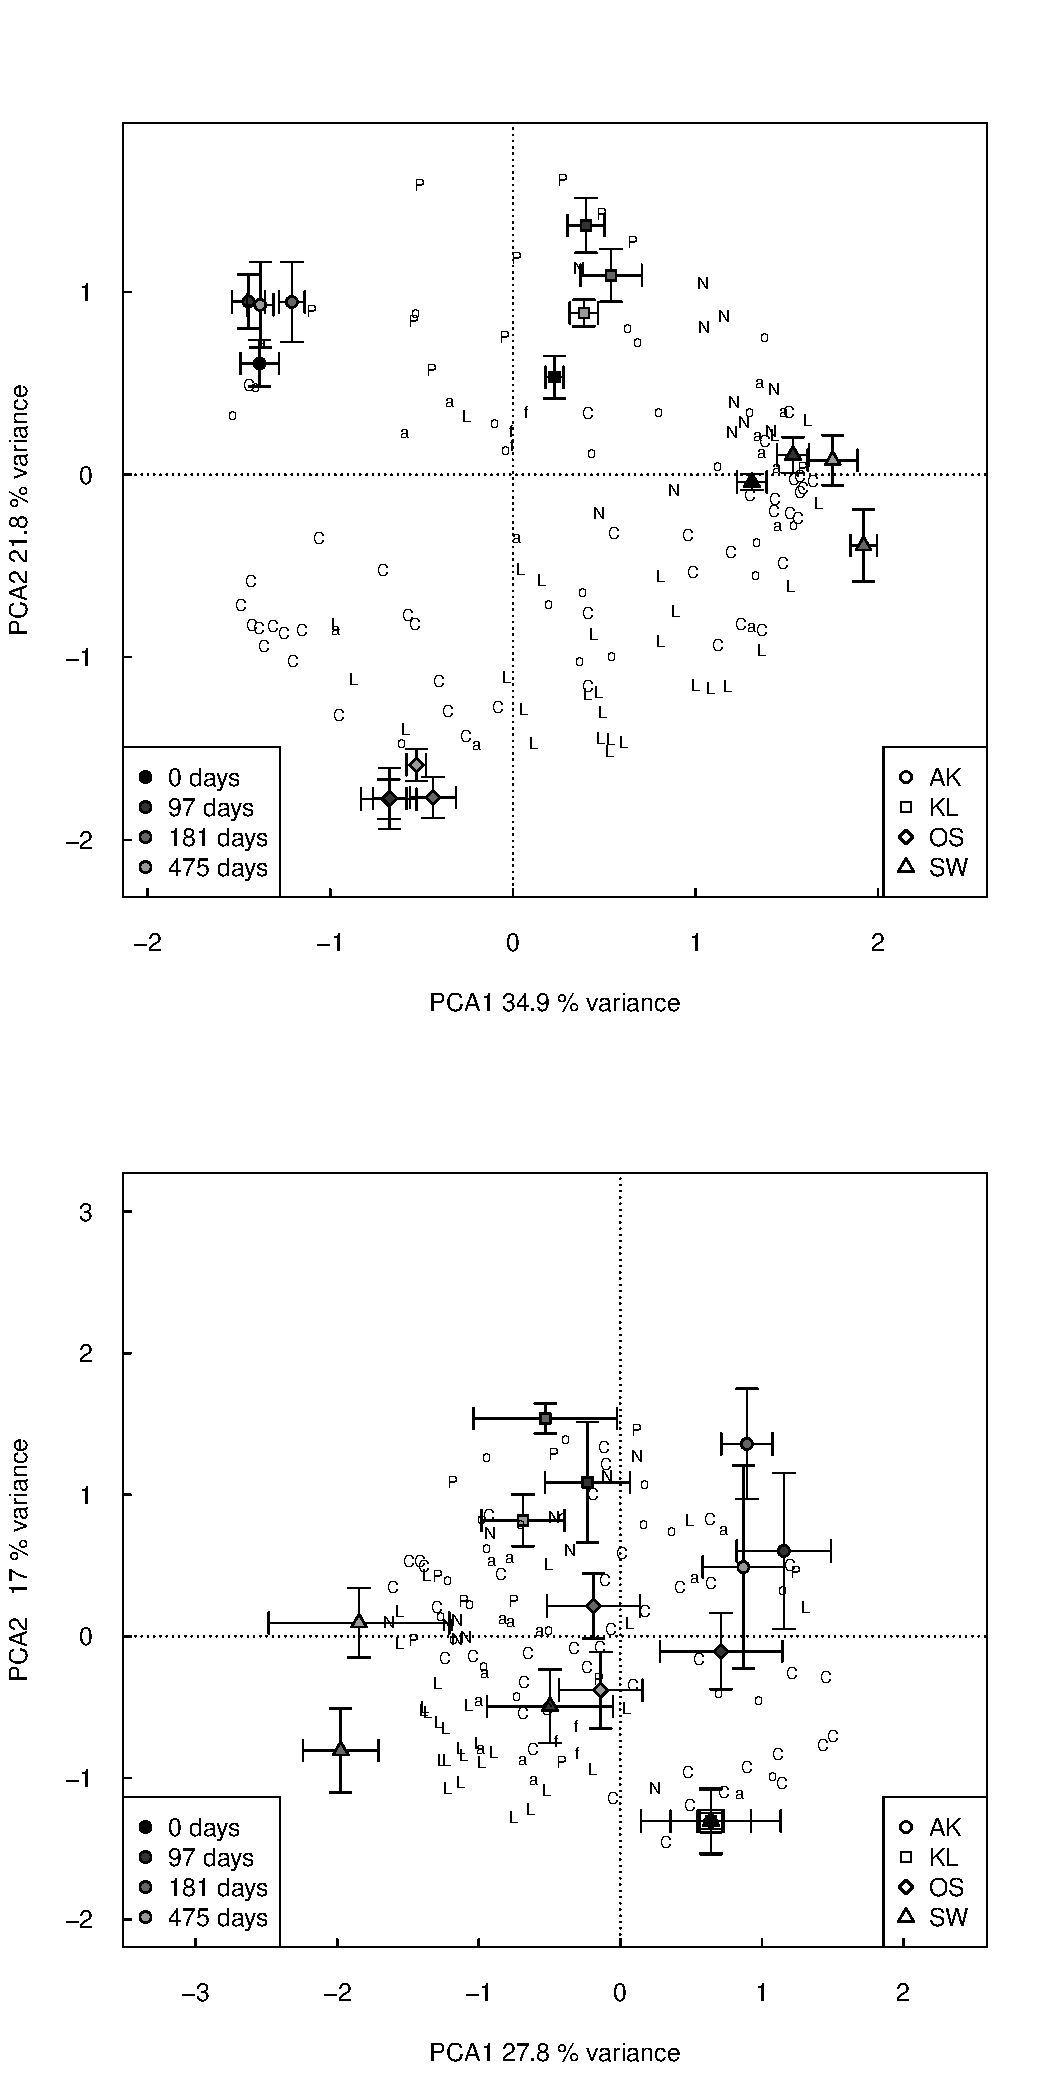
\includegraphics{aap-pca1}
\end{center}
\caption{PCA based on 128 peaks quantified in 74 samples. Error bars indicate standard errors (n=4-5). Letters indicate pyrolysis products:  C - carbohydrates, L - lignin, P - other phenolic compounds, N - N containing compounds,  a - long chained aliphatic compounds (fatty acids, n- alkanes, n-alkenes, phytol}
\label{fig:pca1}
\end{figure*}

\newpage
\begin{figure*}[h!]
\begin{center}
\setkeys{Gin}{width=\textwidth}
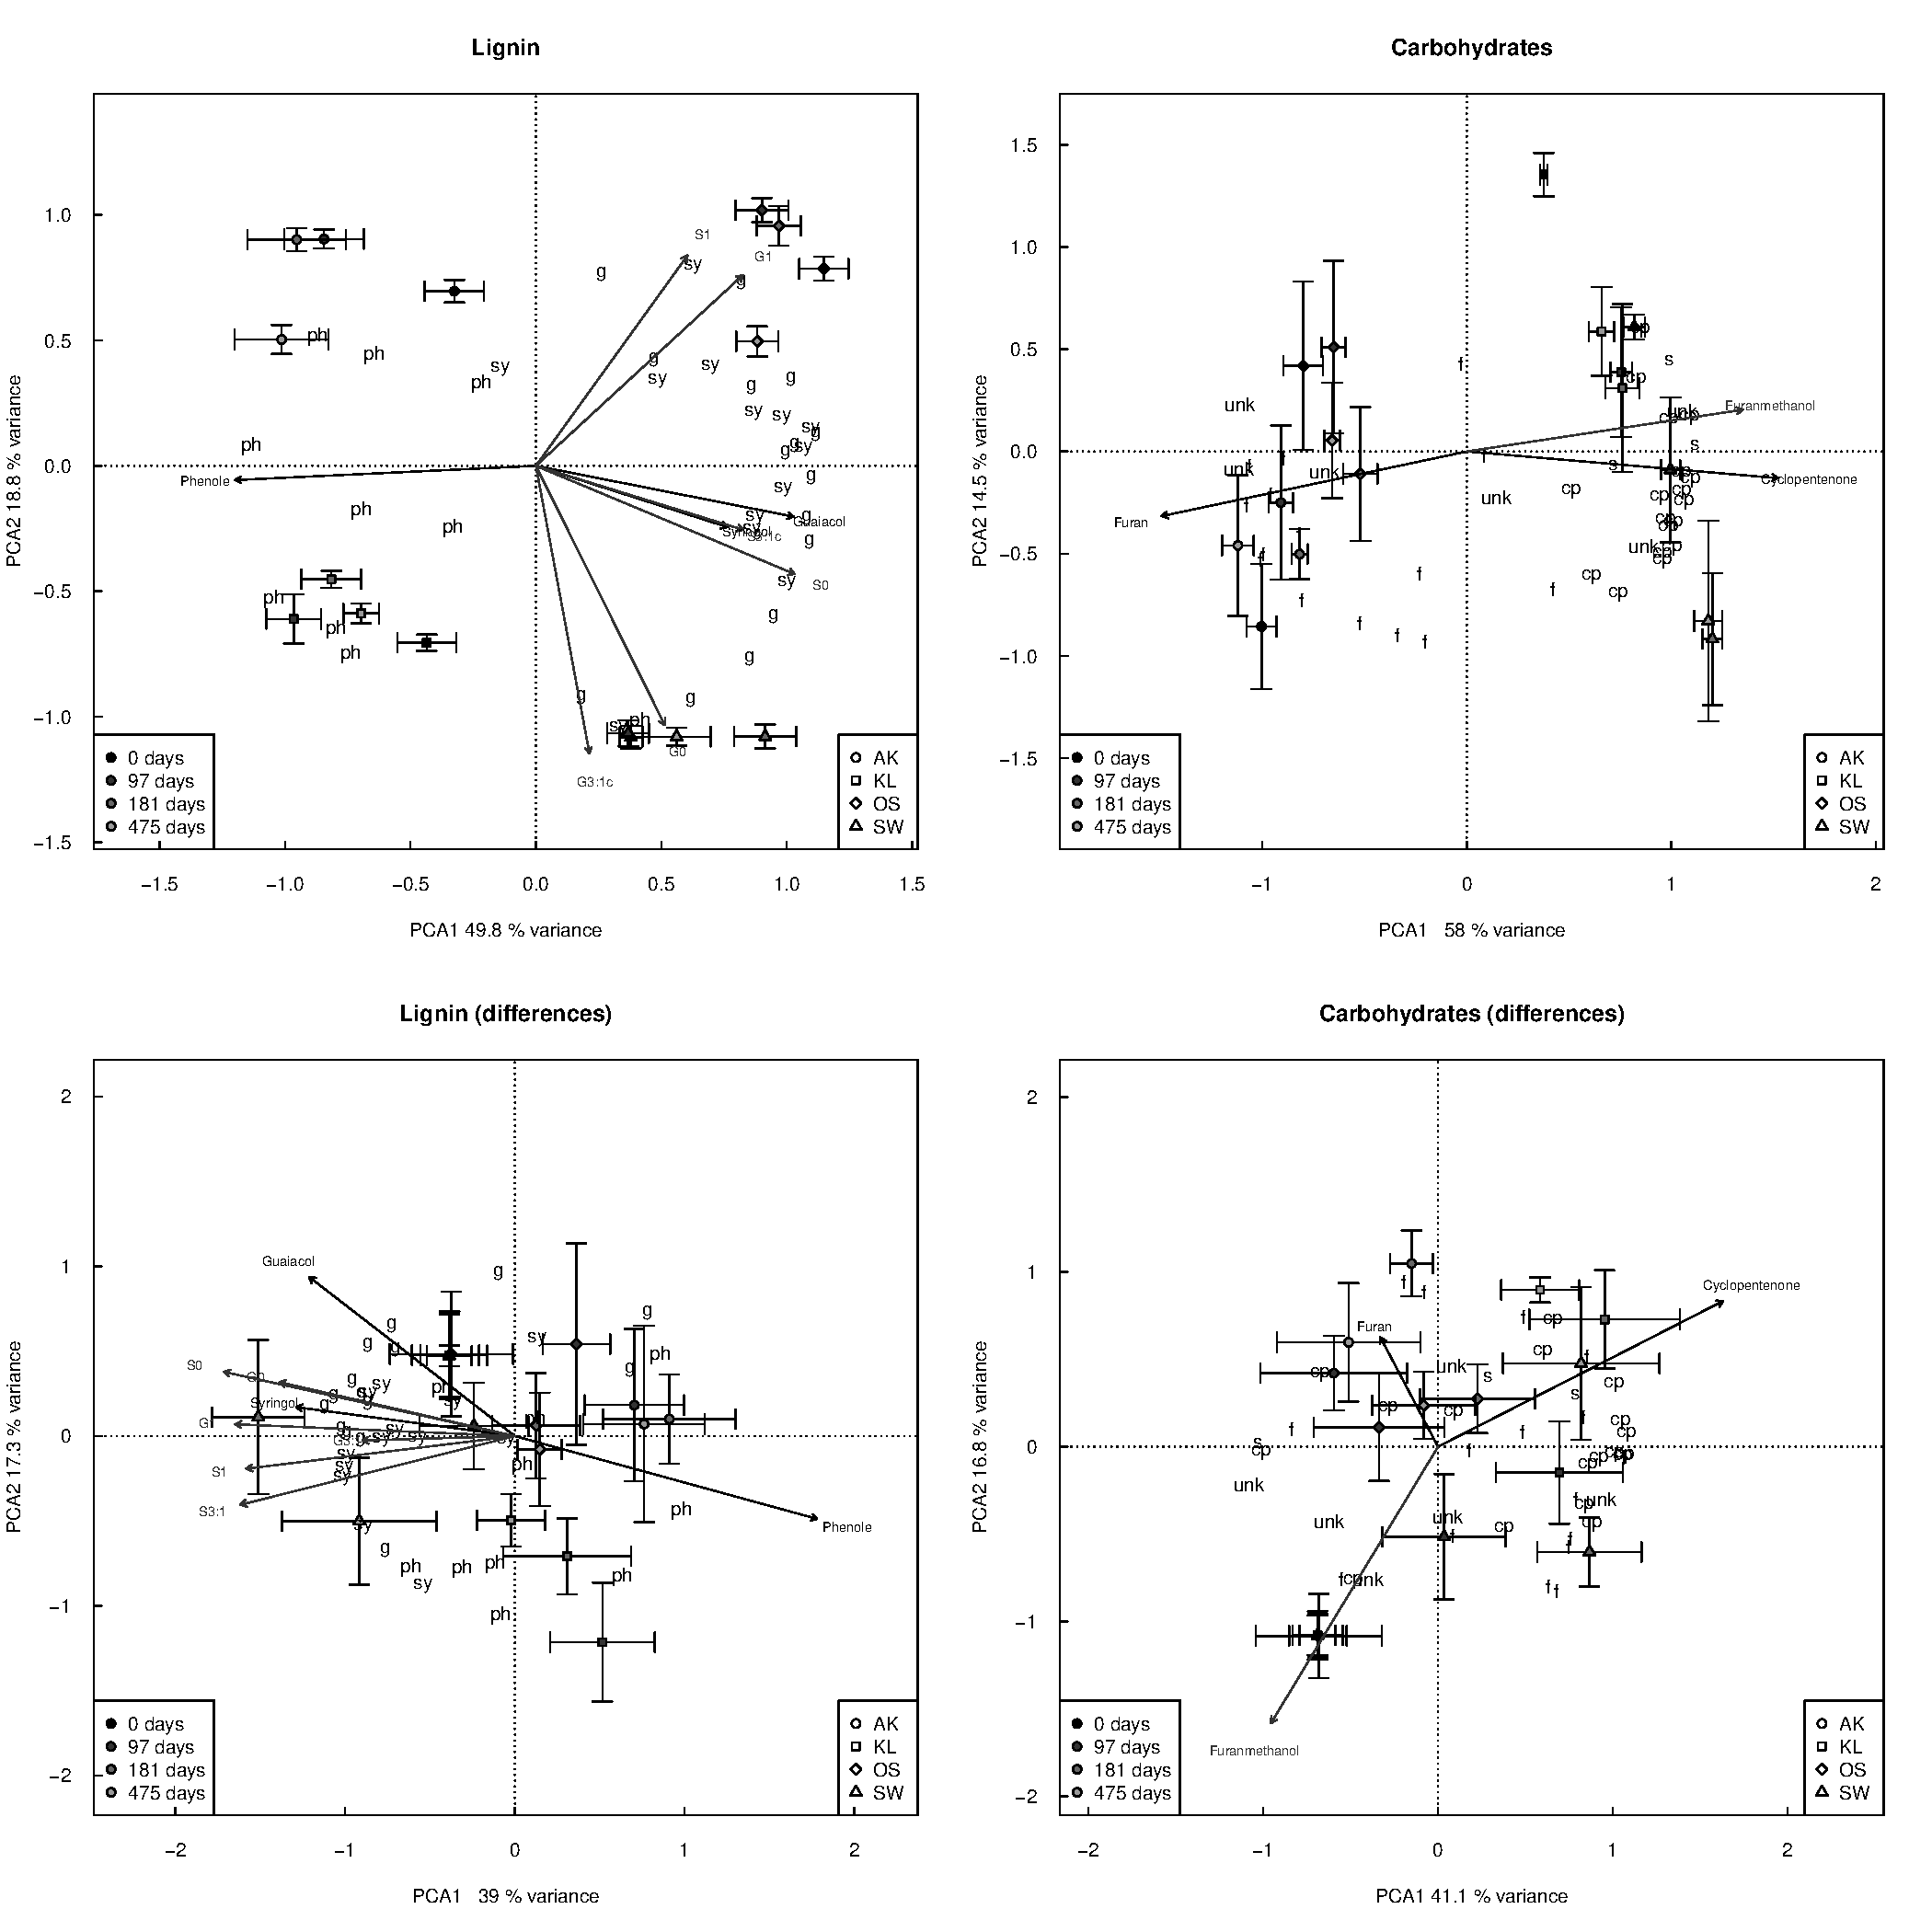
\includegraphics{aap-pcalph}
\end{center}
\caption{The upper left graphs shows a PCA of relative contributions of lignin and phenol pyrolysis products to the sum of these products, the lower left graph shows the difference of this relative contribution to initial contributions. The both graphs on the right hand show the same relations for carbohydrate derrived pyrolysis products. Sample means (n=4-5) and standard errors are stated as indicated in the plot legend. Letters indicate pyrolysis products (g - guaiacol lignin, sy - syringol lignin, ph - phenolic compounds, cp - cyclopentenone-type and f - furan type carbohydrade markers). Black arrows indicate fits for \%TIC sum of compound classes (guaiacol and syringol lignin, other phenolic compounds, furan- and cyclopentenone-type carbohydrate markers), grey arrows indicate selected individual markers (G1/S0 - guaiacol/syringol, G/S1 - methylguaiacol/-syringol, G3:1/S3:1 - Propenylguaiacol/syringol.) The lower graph shows a PCA based on  differences to initial peak abundance.}
\label{fig:pcalph}
\end{figure*}


\newpage
\begin{figure*}[h!]
\begin{center}
\setkeys{Gin}{width=\textwidth}
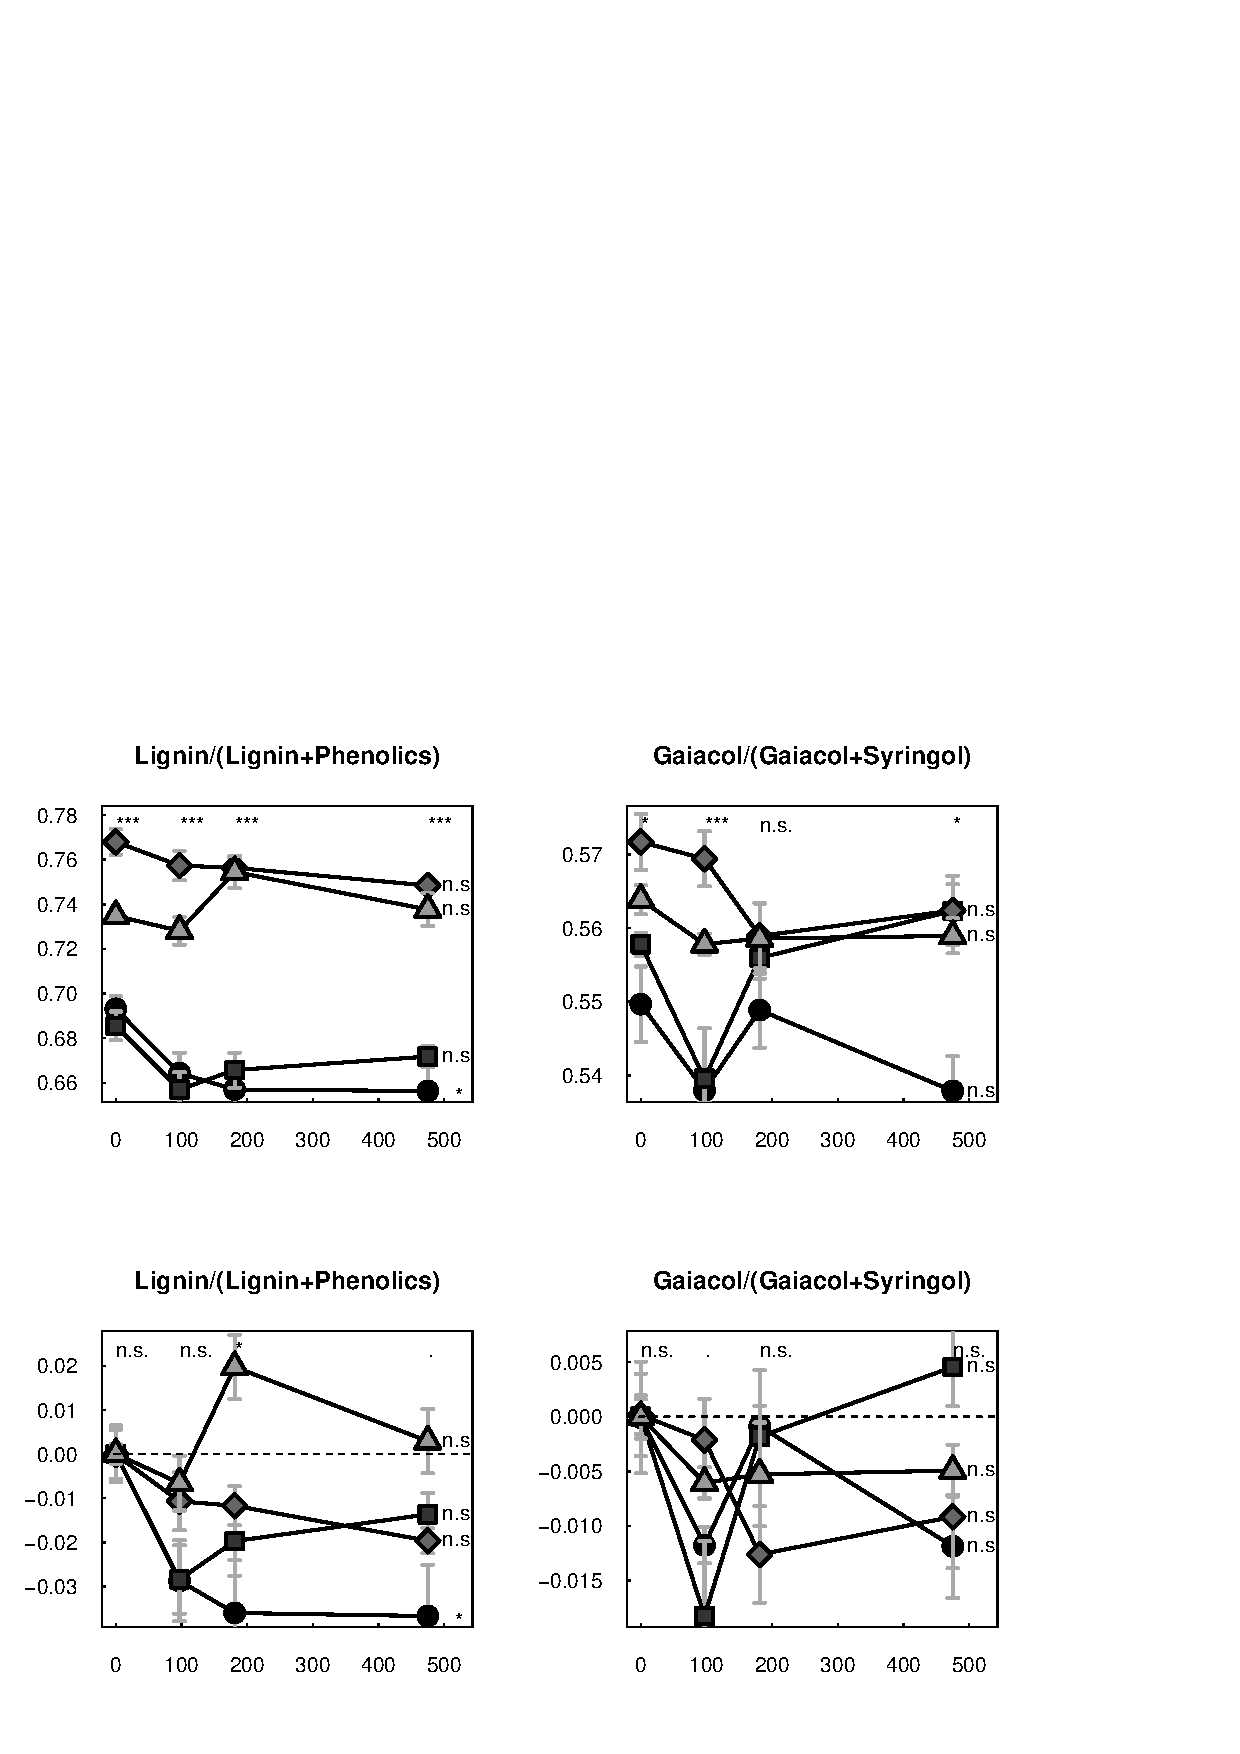
\includegraphics{aap-g2syTS}
\end{center}
\caption{}
\label{fig:gsyph}
\end{figure*}

\begin{figure}
\centering
\setkeys{Gin}{width=\textwidth}
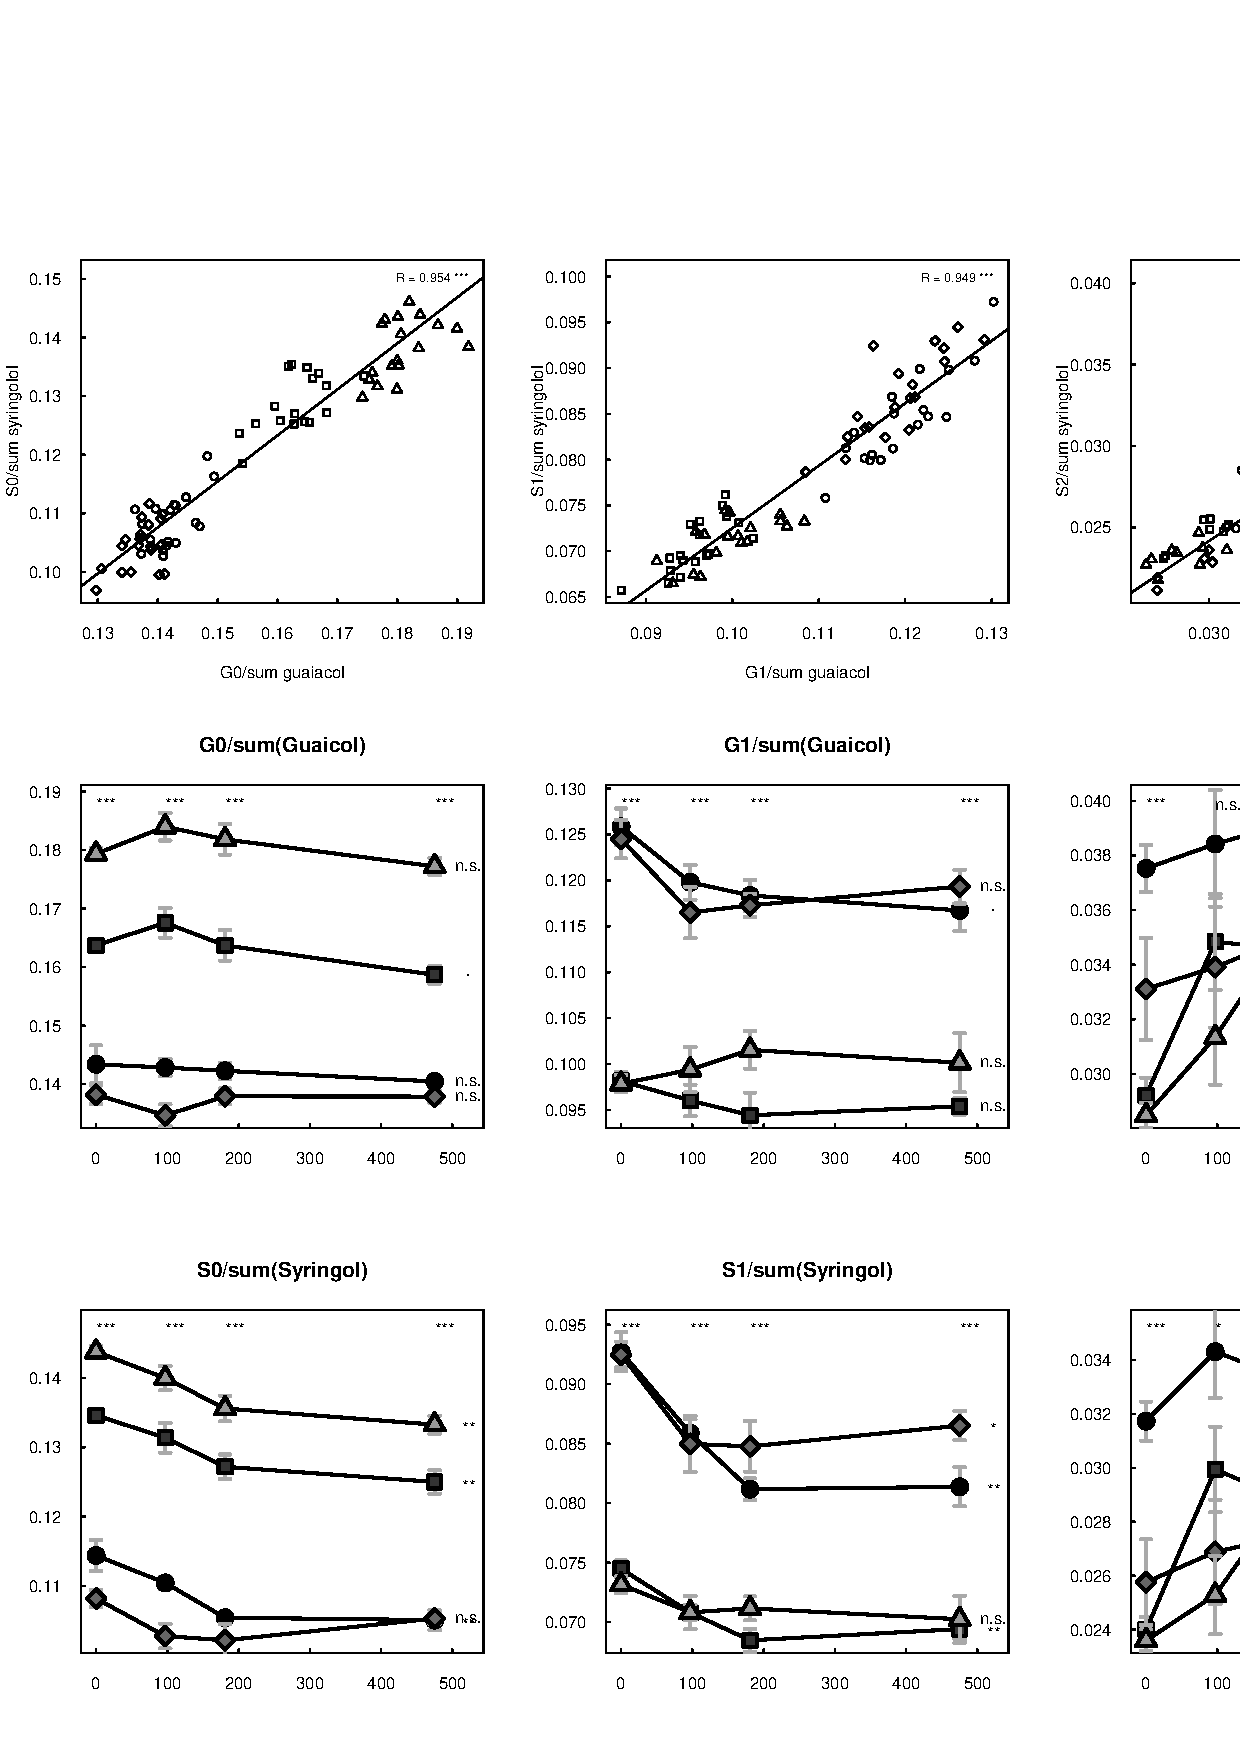
\includegraphics{aap-sidechainratios}
\caption{Lignin side chains occur in the same ratios for both guaiacol and syringol lignin, but differences in the content of -H and -CH$_3$ side chains were found.}
\label{fig:sidechainratios}
\end{figure}

\begin{figure}
\centering
\setkeys{Gin}{width=\textwidth}
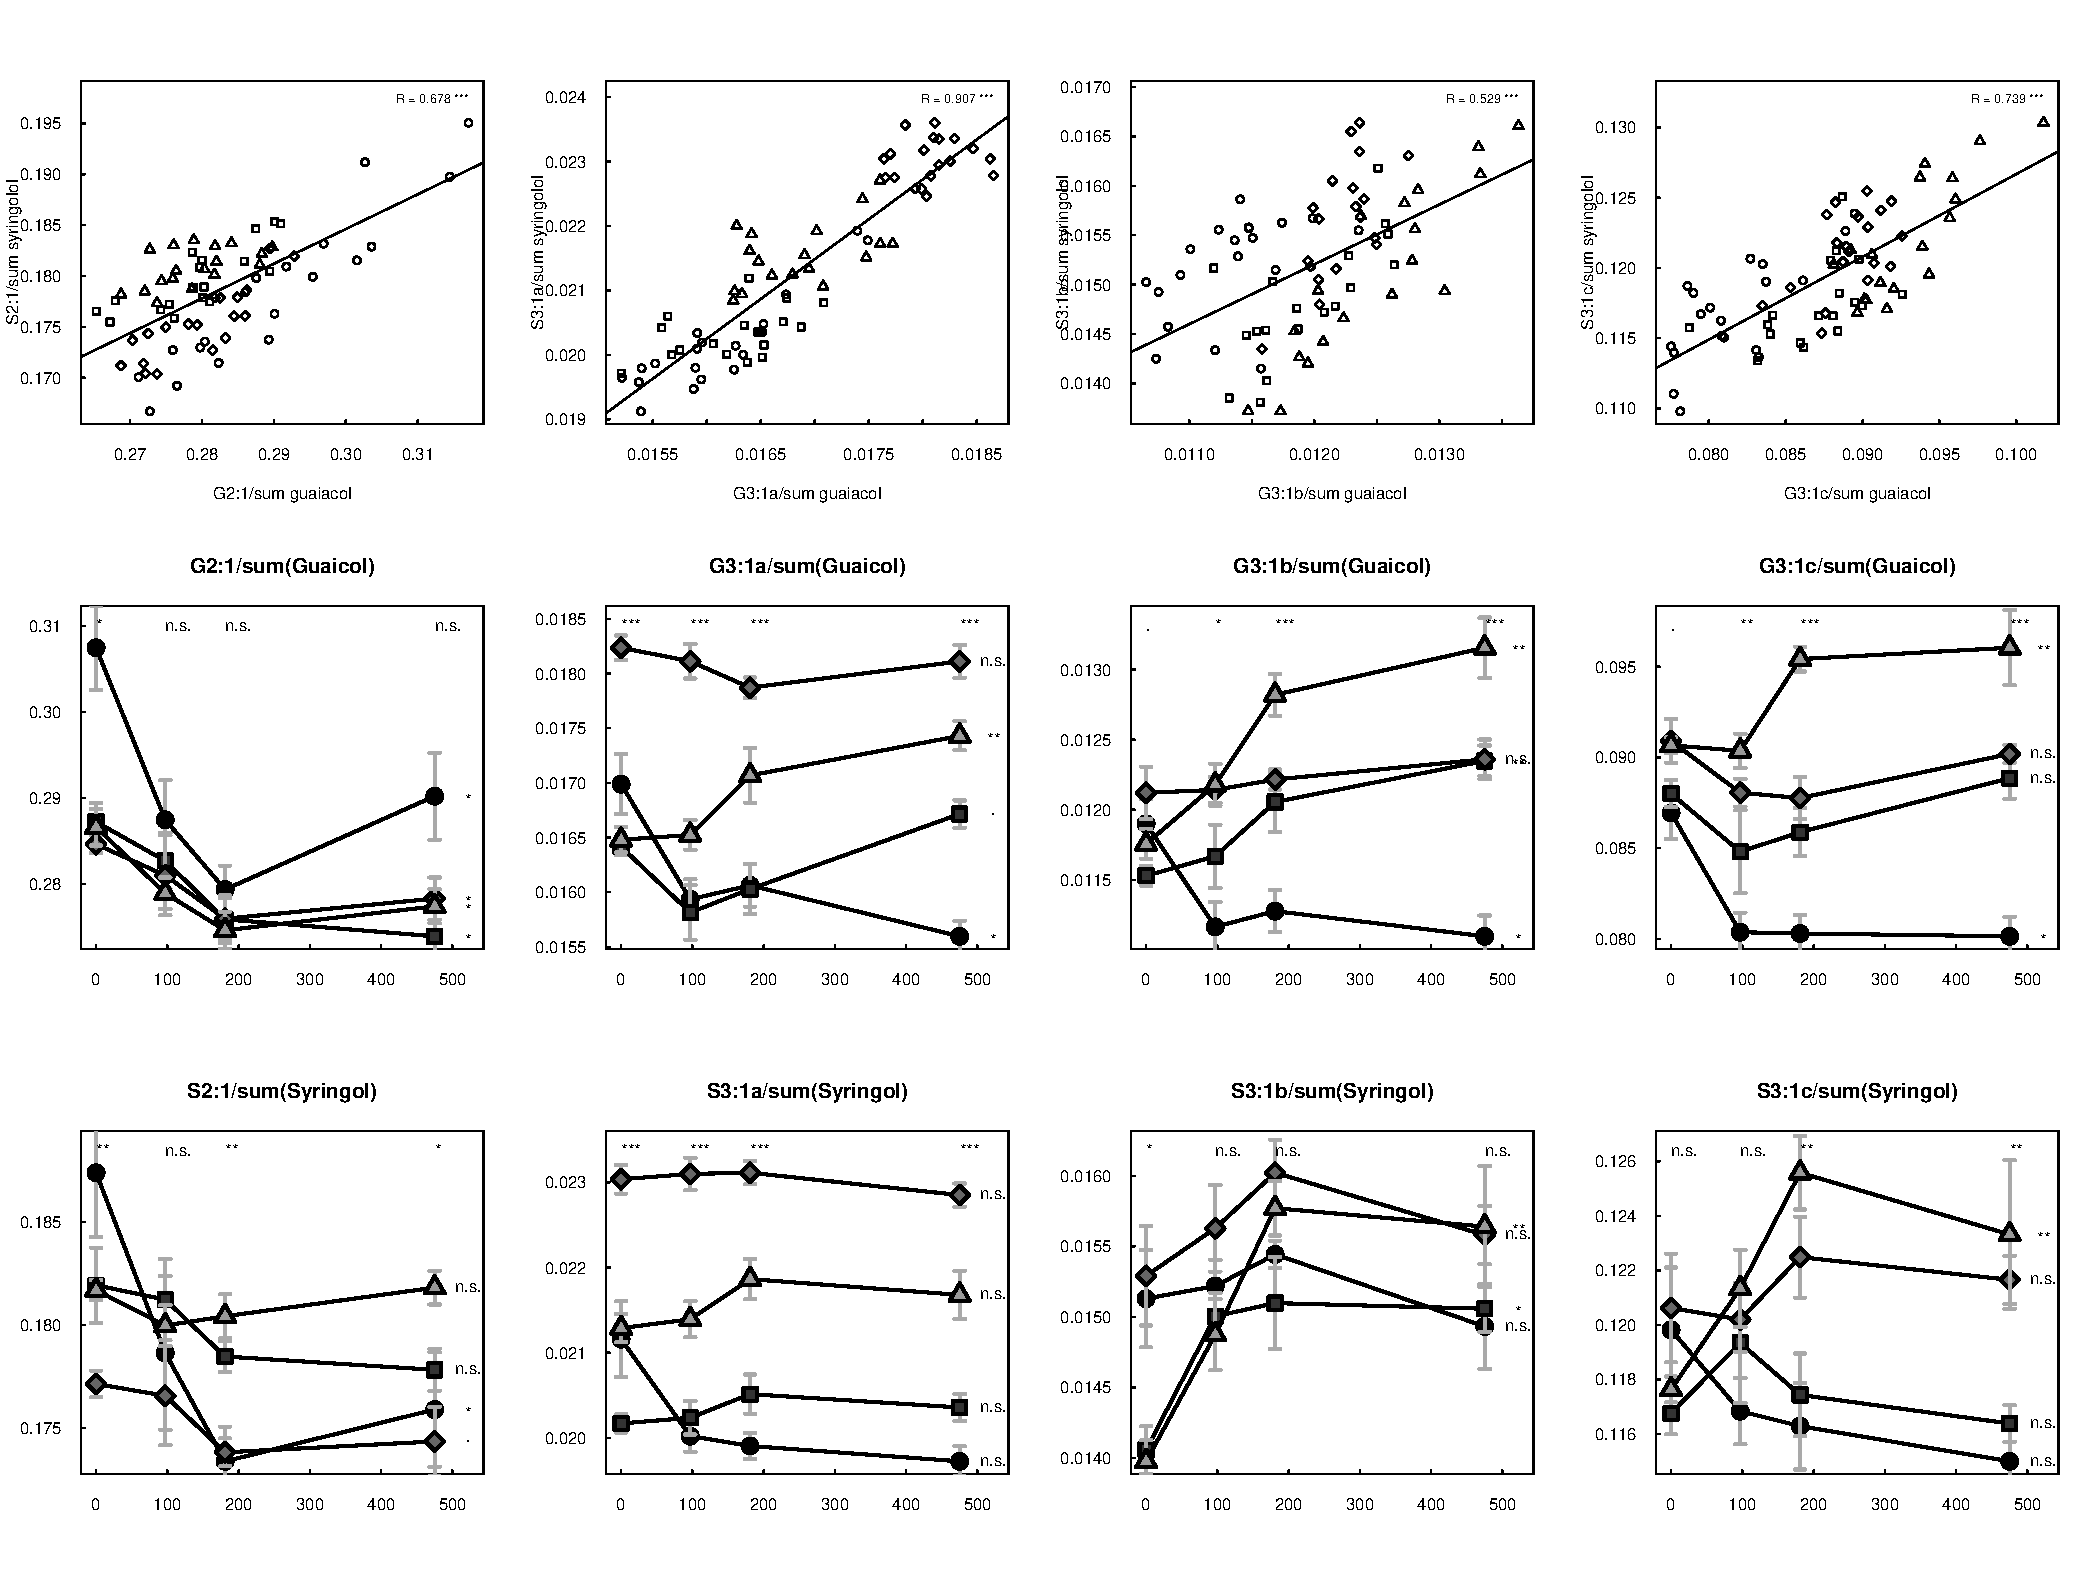
\includegraphics{aap-sidechainratios2}
\caption{Lignin side chains occur in the same ratios for both guaiacol and syringol lignin, but differences in the content of -H and -CH$_3$ side chains were found.}
\label{fig:sidechainratios2}
\end{figure}
\begin{figure}
\centering
\setkeys{Gin}{width=\textwidth}
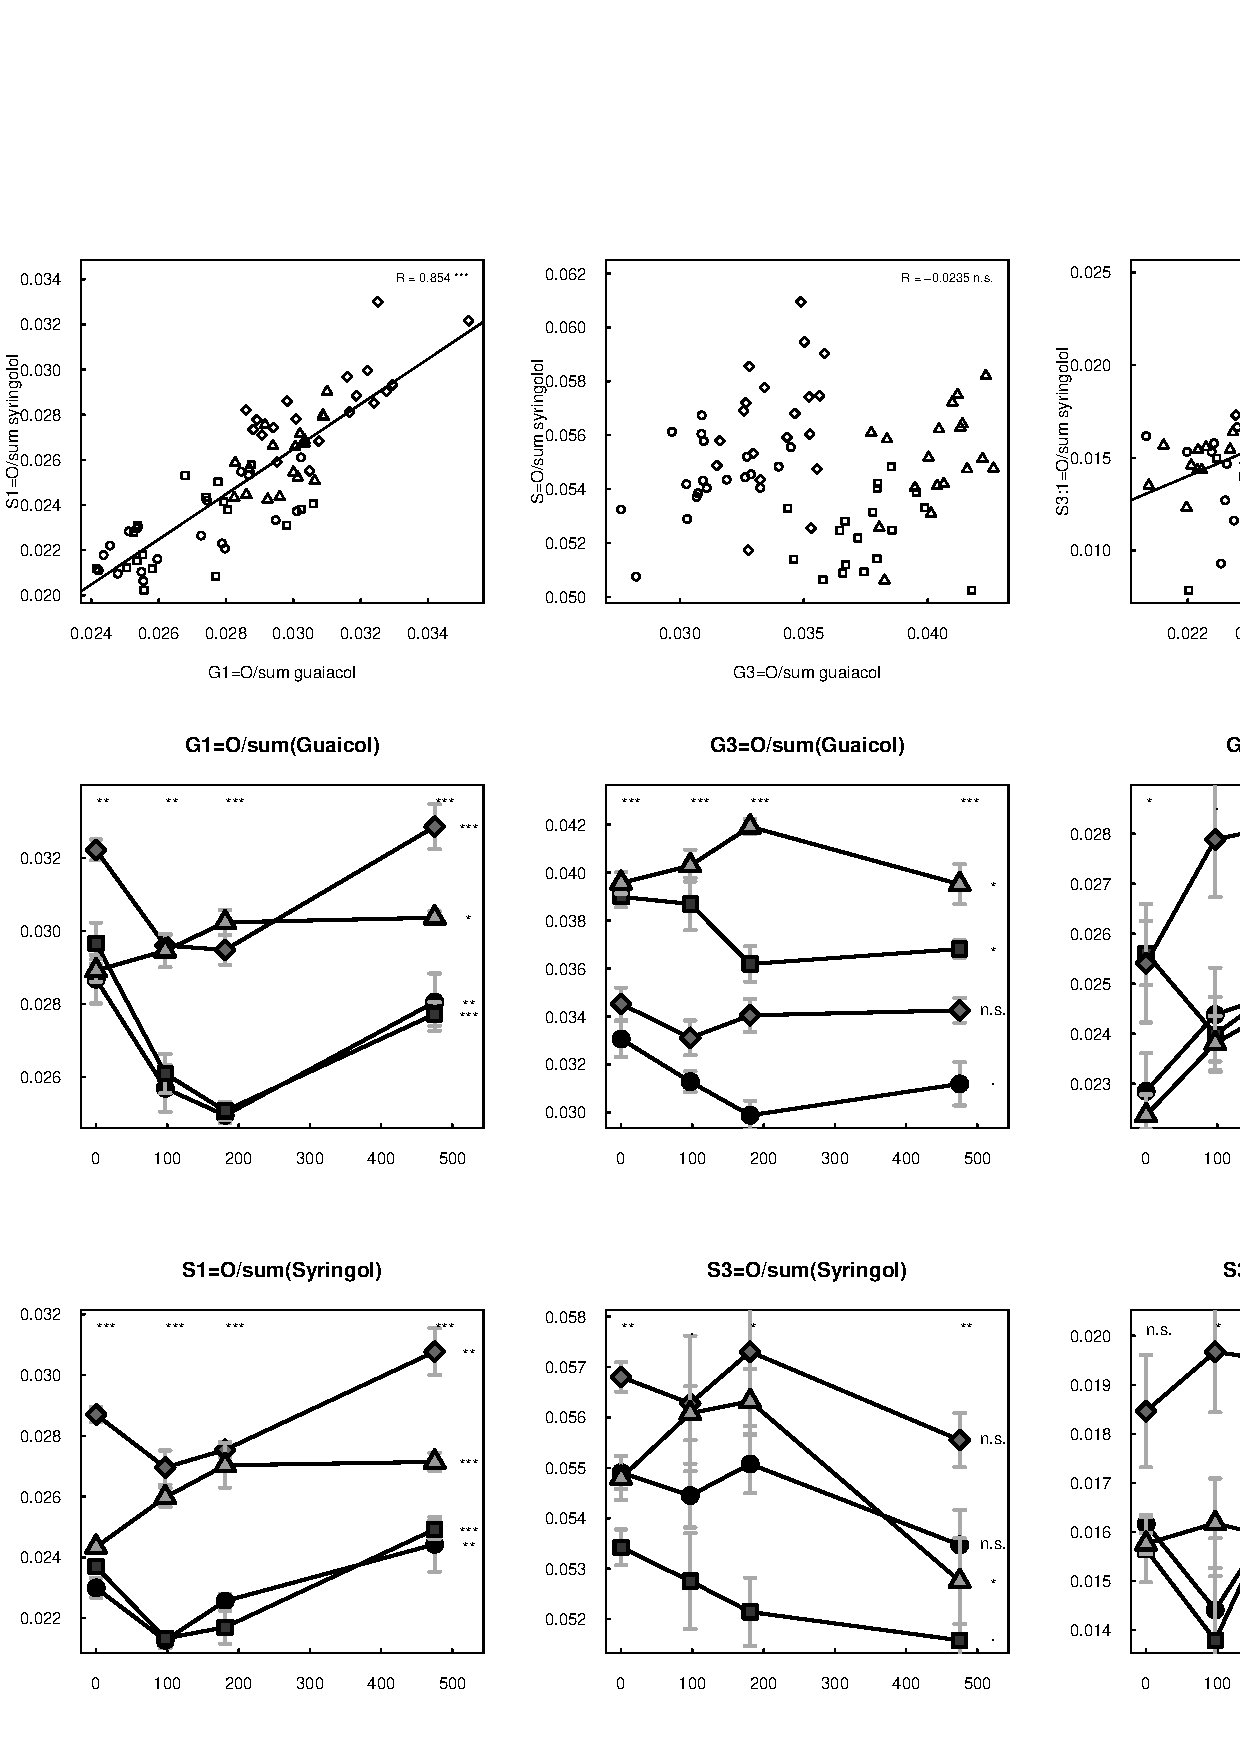
\includegraphics{aap-sidechainratios3}
\caption{Lignin side chains occur in the same ratios for both guaiacol and syringol lignin, but differences in the content of -H and -CH$_3$ side chains were found.}
\label{fig:sidechainratios3}
\end{figure}

\newpage
\begin{figure*}[h!]
\vspace*{2mm}
\begin{center}
\setkeys{Gin}{width=0.8\textwidth}

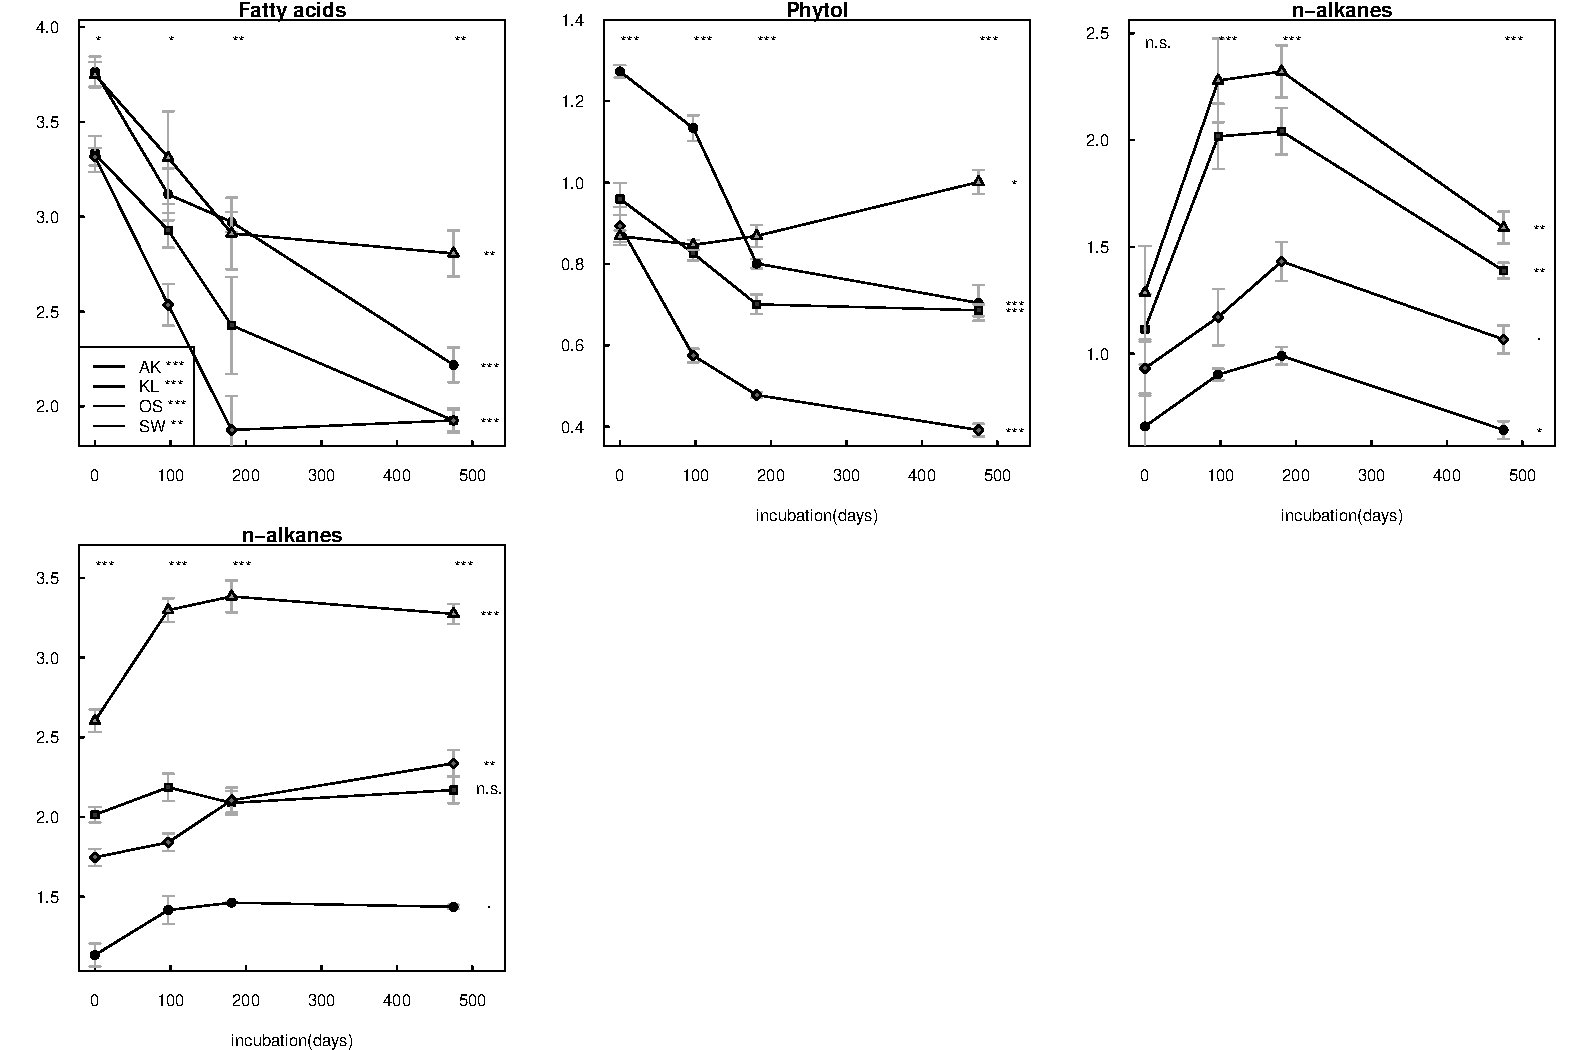
\includegraphics{aap-notlignin}
\end{center}
\caption{Trends for lipophilic compounds found in isolated lignin. Two samples were excluded due to contaminations.}
\label{fig:notlig}
\end{figure*}

\newpage
\begin{figure*}[h!]
\vspace*{2mm}
\begin{center}
\setkeys{Gin}{width=\textwidth}

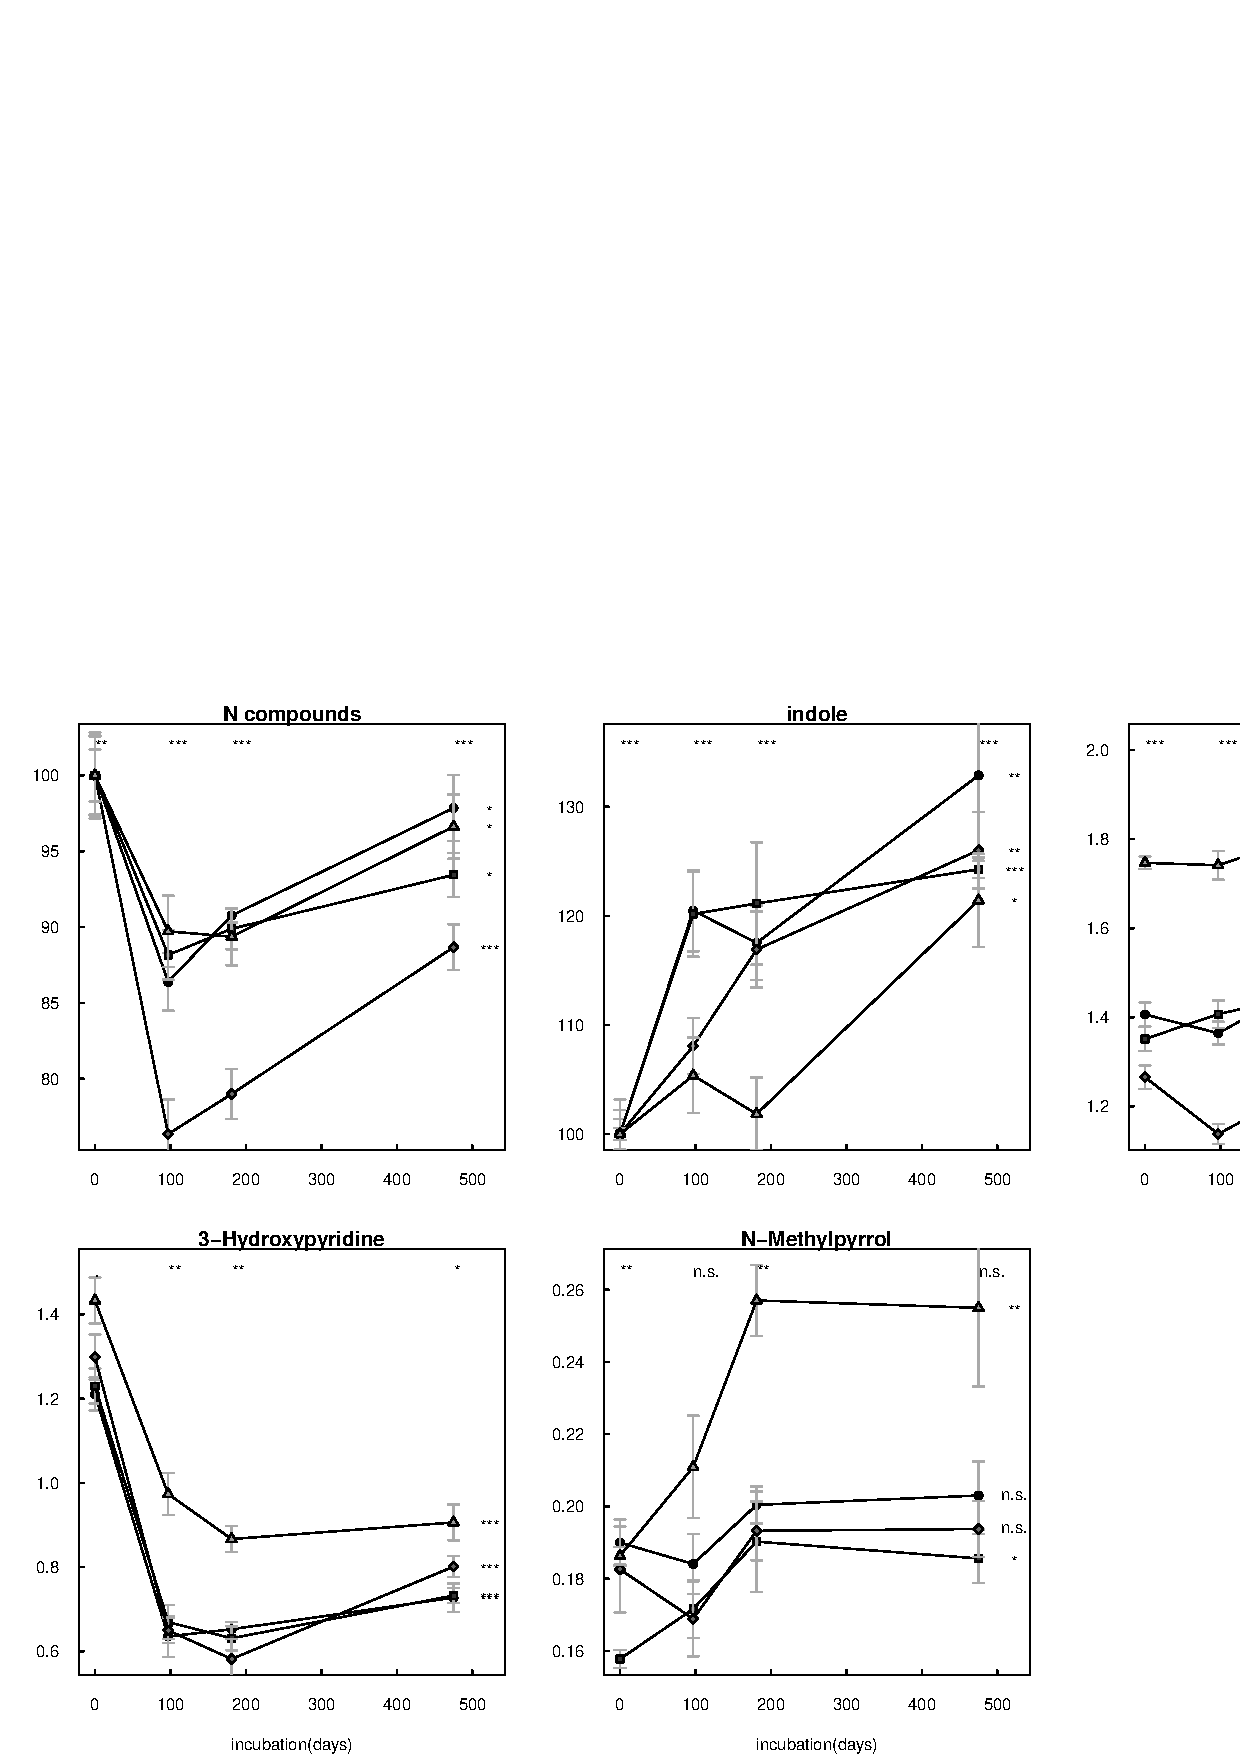
\includegraphics{aap-ncomp}
\end{center}
\caption{Trends for nitrogen compounds found in isolated lignin. Two samples were excluded due to contaminations.}
\label{fig:npeaks}
\end{figure*}


%\begin{figure}[p!]
%  \caption{G/Sy ratio for 5 pairs of compounds with different side chains.}
%  \centering
%    \includegraphics[width=0.5\textwidth]{G_Sy_ratio.pdf}
%\end{figure}


\newpage
% latex table generated in R 2.12.1 by xtable 1.5-6 package
% Thu Oct  6 13:47:08 2011
\begin{table}[h!]
\begin{center}
\caption{Lignin derrived and other phenolic pyrolysis products}
\label{tab:phprod}
{\tiny
\begin{tabular}{ccccccc}
  \hline
 & Name & RT & MW & integrated framents & Origin & Class \\ 
  \hline
1 & Guaiacol & 18.87 & 124 & 109+124 & L & g \\ 
  2 & Methylguaiacol & 20.32 & 138 & 123+138 & L & g \\ 
  3 & Ethylguaiacol & 21.40 & 152 & 137+152 & L & g \\ 
  4 & Propenylguaiacol & 23.29 & 164 & 149+164 & L & g \\ 
  5 & Vinylguaiacol & 23.69 & 150 & 135+150 & L & g \\ 
  6 & Propenylguaiacol & 24.48 & 164 & 149+164 & L & g \\ 
  7 & Syringol & 24.58 & 154 & 139+154 & L & sy \\ 
  8 & Propenylguaiacol & 25.66 & 164 & 149+164 & L & g \\ 
  9 & Methylsyringol & 25.67 & 168 & 153+168 & L & sy \\ 
  10 & Ethylsysringol & 26.39 & 182 & 167+182 & L & sy \\ 
  11 & Propenylsyringol & 27.97 & 194 & 179+194 & L & sy \\ 
  12 & Vinylsyringol & 28.37 & 180 & 165+180 & L & sy \\ 
  13 & Guaiacolaldehyde & 28.40 & 152 & 109+152 & L & g \\ 
  14 & Propylguaiacol & 28.72 & 166 & 137+166 & L & g \\ 
  15 & Oxo-hydroxy-etylguaiacol & 28.77 & 182 & 182 & L & g \\ 
  16 & Propenylsyringol & 28.91 & 194 & 179+194 & L & sy \\ 
  17 & Oxo-ethylguaiacol & 29.20 & 166 & 151+166 & L & g \\ 
  18 & Oxo-propylguaiacol & 29.36 & 180 & 137+180 & L & g \\ 
  19 & Propenylsyringol & 30.16 & 194 & 194+179 & L & sy \\ 
  20 & Syringolaldehyde & 32.68 & 182 & 139+182 & L & sy \\ 
  21 & Oxo-hydroxy-ethylsyringol & 32.80 & 212 & 212 & L & sy \\ 
  22 & Guaiacolacetic acid & 32.88 & 182 & 137+182 & L & g \\ 
  23 & Propylsyringol & 33.15 & 196 & 181+196 & L & sy \\ 
  24 & Oxo-propylsyringol & 33.32 & 210 & 167+210 & L & sy \\ 
  25 & Oxopropenylguaiacol & 35.30 & 178 & 135+178 & L & g \\ 
  26 & Hydroxypropenylguaiacol & 37.10 & 137+180 & 180 & L & g \\ 
  27 & Syringolacetic acid & 38.78 & 212 & 212 & L & sy \\ 
  28 & Oxo-propenylsyringol & 43.06 & 208 & 165+208 & L & sy \\ 
  29 & Phenol & 21.02 & 94 & 65+66+94 & Ph & ph \\ 
  30 & 4-Methylphenol & 22.11 & 108 & 107+108 & Ph & ph \\ 
  31 & 3-Methylphenol & 22.22 & 108 & 107+108 & Ph & ph \\ 
  32 & Ethylphenol & 23.38 & 122 & 107+122 & Ph & ph \\ 
  33 & Propenylphenol & 26.93 & 134 & 133+134 & Ph & ph \\ 
  34 & Propenylphenol & 27.76 & 134 & 133+134 & Ph & ph \\ 
  35 & Propylphenol & 31.11 & 136 & 151+166 & Ph & ph \\ 
  36 & Butylphenol? & 31.86 & 150 & 107+150 & Ph & ph \\ 
  37 & 4-Hydroxybenzaldehyde & 32.70 & 122 & 121+122 & Ph & ph \\ 
  38 & Hydroquinone & 33.40 & 110 & 81+110 & Ph & ph \\ 
   \hline
\end{tabular}
}
\end{center}
\end{table}
\newpage

% latex table generated in R 2.12.1 by xtable 1.5-6 package
% Thu Oct  6 13:47:08 2011
\begin{table}[h!]
\begin{center}
\caption{Carbohydrate derrived pyrolysis products}
\label{tab:chprod}
{\tiny
\begin{tabular}{ccccccc}
  \hline
 & Name & RT & MW & integrated framents & Origin & Class \\ 
  \hline
1 & Acetaldehyde & 2.06 & 44 & 29+44 & C & cp \\ 
  2 & Furan & 2.35 & 68 & 39+68 & C & f \\ 
  3 & Methylfuran & 2.74 & 82 & 81+82 & C & f \\ 
  4 & Methylfuran & 2.91 & 82 & 81+82 & C & f \\ 
  5 & Dimethylfuran & 3.43 & 96 & 95+96 & C & f \\ 
  6 & Dimethylfuran & 3.66 & 96 & 95+96 & C & f \\ 
  7 & Vinylfuran & 5.01 & 94 & 65+94 & C & f \\ 
  8 & Unknown furan & 6.36 & 108 & 107+108 & C & f \\ 
  9 & Cyclopentanone & 6.99 & 105? & 84+105? & C & cp \\ 
  10 & Methylfuran & 7.62 & 82 & 53+82+83 & C & f \\ 
  11 & 2-Oxopropanoic acid, methylester & 7.92 & 102 & 43+102 & C & s \\ 
  12 & 1-Hydroxypropanone & 9.24 & 74 & 43 & C & s \\ 
  13 & 2-Cyclopenten-1-one & 10.26 & 82 & 53+54+52 & C & cp \\ 
  14 & 2-Methyl-2-cyclopenten-1-one & 10.51 & 96 & 53+96 & C & cp \\ 
  15 & 1-Hydroxy-2-propanone & 10.69 & 88 & 57+88 & C & cp \\ 
  16 & Unknown & 11.38 & unk & 65+66+94 & C & cp \\ 
  17 & 3-Furaldehyd & 11.57 & 96 & 95+96 & C & f \\ 
  18 & 2(5H)Furanon & 11.69 & 98 & 55+98 & C & f \\ 
  19 & Propanoic acid, methylester & 12.10 & 102 & 43+102 & C & s \\ 
  20 & 2-Furaldehyd & 12.22 & 96 & 95+96 & C & f \\ 
  21 & Acetylfuran & 12.99 & 110 & 95+110 & C & cp \\ 
  22 & 3-Methyl-cyclopentanone & 13.31 &  & 67+96 & C & cp \\ 
  23 & Dimethylcyclopentenone & 13.69 & 110 & 67+95+110 & C & cp \\ 
  24 & 5-Methyl-2-furancarboxaldehyde & 14.23 & 110 & 109+110 & C & f \\ 
  25 & 2-Cyclopenten-1,4-dione & 14.44 & 96 & 54+68+96 & C & cp \\ 
  26 & Butyrolactone & 15.22 & 86 & 56+86 & C & cp \\ 
  27 & Unknown & 15.56 & ? & ? & C & cp \\ 
  28 & Furanmethanol & 15.61 & 98 & 98 & C & cp \\ 
  29 & 5-Methyl-2(5H)-furanone & 16.06 & 98 & 55+98 & C & f \\ 
  30 & Unknown & 16.17 & unk & 110 & C & cp \\ 
  31 & 1,2-Cylopentandione & 17.51 & 98 & 55+98 & C & cp \\ 
  32 & Unknown & 17.67 & unk & 42+70 & C & cp \\ 
  33 & 2-Hydroxy-3-methyl-2-cyclopenten-1-one & 18.14 & 98 & 98 & C & cp \\ 
  34 & 3-Methy-l1,2-cyclopentanedione & 18.42 & 112 & 69+112 & C & cp \\ 
  35 & Unknown & 19.06 & unk & 58+86+114 & C & unk \\ 
  36 & Unknown & 19.35 & unk & 98+126 & C & unk \\ 
  37 & Unknown & 21.77 & unk & 116 & C & unk \\ 
  38 & Unknown & 22.33 & unk & 44 & C & unk \\ 
  39 & Unknown & 26.18 & unk & 57+69 & C & unk \\ 
  40 & 5-Hydroxymethylfuran1--carboxaldehyde & 27.51 & 126 & 97+126 & C & f \\ 
  41 & Unknown & 31.67 & unk & 73+135 & C & unk \\ 
  42 & Laevoglucosan & 40.44 & 172 & 60+73 & C & f \\ 
   \hline
\end{tabular}
}
\end{center}
\end{table}


\newpage
% latex table generated in R 2.12.1 by xtable 1.5-6 package
% Thu Oct  6 13:47:08 2011
\begin{table}[h!]
\begin{center}
\caption{Other pyrolysis products quantified}
\label{tab:nprod}
{\tiny
\begin{tabular}{ccccccc}
  \hline
 & Name & RT & MW & integrated framents & Origin & Class \\ 
  \hline
1 & 25:0 &  &  &  & Cut & cut0 \\ 
  2 & 25:1 &  &  &  & Cut & cut1 \\ 
  3 & 27:0 &  &  &  & Cut & cut0 \\ 
  4 & 27:1 &  &  &  & Cut & cut1 \\ 
  5 & 29:0 &  &  &  & Cut & cut0 \\ 
  6 & 29:1 &  &  &  & Cut & cut1 \\ 
  7 & Myristic acid (14:0) & 2.35 & 68 & 39+68 & lip & fa \\ 
  8 & Palmitic acid (16:0) & 2.74 & 82 & 81+82 & lip & fa \\ 
  9 & Stearuc acid (18:0) & 2.91 & 82 & 81+82 & lip & fa \\ 
  10 & N-methyl-pyrrol & 6.15 & 81 & 80+81 & N & N-me-pyr \\ 
  11 & Pyridine & 6.90 & 95 & 52+79+95 & N & p \\ 
  12 & Methylpyridine & 7.50 & 93 & 66+92+93 & N & p \\ 
  13 & Methylpyridine & 7.54 & 93 & 66+92+93 & N & p \\ 
  14 & methylpyridine & 9.02 & 93 & 66+93 & N & p \\ 
  15 & Pyrrol & 13.11 & 67 & 39+41+67 & N & p \\ 
  16 & Methylpyrrol & 13.81 & 81 & 80+81 & N & p \\ 
  17 & Methylpyrrol & 14.10 & 81 & 80+81 & N & p \\ 
  18 & 3-Hydroxypyridine & 26.52 & 95 & 67+95 & N & pyridol \\ 
  19 & Indole & 26.85 & 117 & 89+117 & N & ind \\ 
  20 & Methylindole & 27.42 & 131 & 130+131 & N & ind \\ 
  21 & Aceton & 2.46 & 58 & 43 & non & short \\ 
  22 & 2-Propenal & 2.60 & 56 & 55+56 & non & short \\ 
  23 & Methanol & 2.88 & 32 & 29+31+32 & non & short \\ 
  24 & 3-Buten-2-one & 3.39 & 70 & 55+70 & non & short \\ 
  25 & 2,3-Butandione & 3.67 & 86 & 69+86 & non & short \\ 
  26 & 3-Penten-2-one & 3.89 & 86 & 69+86 & non & short \\ 
  27 & Toluene & 4.54 & 92 & 91+92 & non & ar \\ 
  28 & 2-Butanal & 4.56 & 70 & 69+70 & non & short \\ 
  29 & 2,3-Pentadione & 4.77 & 100 & 57+100 & non & short \\ 
  30 & Hexanal & 5.16 & 82 & 56+72+82 & non & short \\ 
  31 & Xylene & 5.94 & 106 & 91+105+106 & non & ar \\ 
  32 & Xylene & 6.09 & 106 & 91+105+106 & non & ar \\ 
  33 & Xylene & 6.20 & 106 & 91+105+106 & non & ar \\ 
  34 & Xylene & 6.99 & 105? & 84+105? & non & ar \\ 
  35 & Limonene & 7.22 & ? & 93 & non & ter \\ 
  36 & 1-Penten-3-one & 11.28 & 84 & 55+84 & non & short \\ 
  37 & Methoxytoluene & 11.78 & 122 & 121+122 & non & ar \\ 
  38 & Indene & 12.64 & 116 & 115+116 & non & ar \\ 
  39 & Benzaldehyde & 13.35 & 106 & 77+106 & non & ar \\ 
  40 & 1-Methyl-4-methoxybenzene & 15.98 & ? & ? & non & ar \\ 
  41 & Phytol & 20.00 & ? & 95+123 & phytol & phytol \\ 
  42 & Unknown & 20.85 & unk & ? & unk & unk \\ 
  43 & Unknown & 20.86 & unk & ? & unk & unk \\ 
  44 & Unknown & 22.43 & unk & 98+128 & unk & unk \\ 
  45 & Unknown aliphatic & 22.82 & unk & 58+71 & unk & al \\ 
  46 & Hexan2,4dion & 23.92 & 114 & 56+84+114 & unk & o \\ 
  47 & Dihydrobenzofuran & 26.19 & 120 & 91+119+120 & unk & bf \\ 
  48 & Unknown & 27.76 & unk & 138 & unk & unk \\ 
   \hline
\end{tabular}
}
\end{center}
\end{table}


\end{document}

%%
%% End of file `elsarticle-template-1a-num.tex'.
